\documentclass[]{article} 
\usepackage{pgfplots} 
\usepgfplotslibrary{external} 
\tikzexternalize 
\usepgfplotslibrary{fillbetween}
\usepackage{tikz} 
\usepackage{amsmath} 
\usepackage{pgfplots} 
\usetikzlibrary{calc} 
\pgfplotsset{compat = newest,every x tick label/.append style={font=\scriptsize,color = white},every y tick label/.append style={font=\scriptsize,color = white}, every axis plot post/.style={line join=round}}

\begin{document} 
	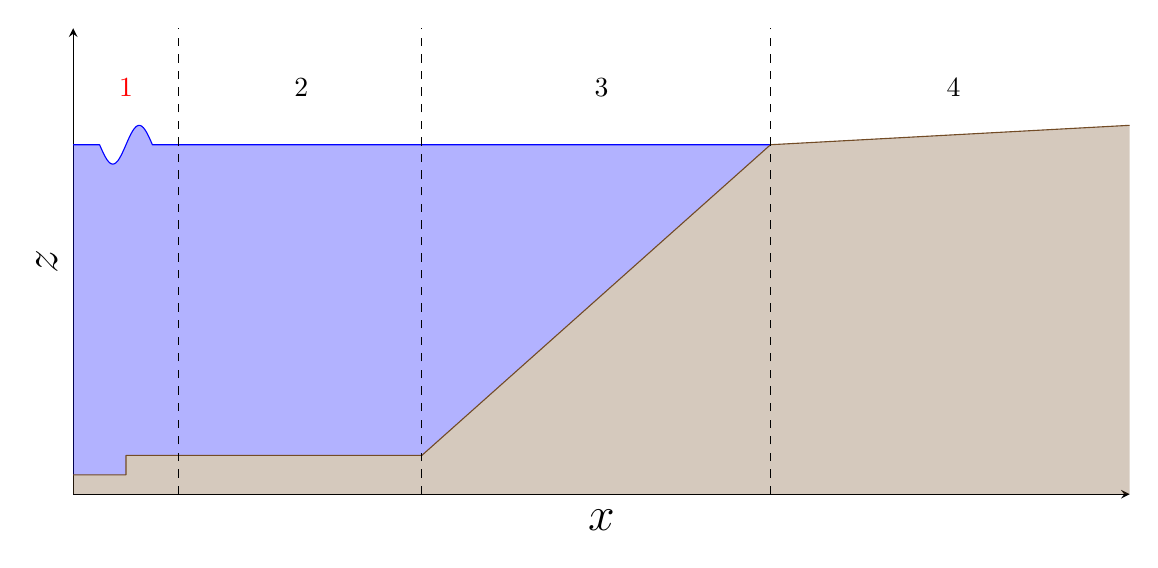
\begin{tikzpicture} 
	\begin{axis}[ 
	width = 0.7\textwidth,
	label style={font=\LARGE},
	axis lines=left, xtick=\empty,
	ytick={-1},
	clip mode=individual,
	xmin=0, 
	xmax=1, 
	width = 15cm,
	height = 7.5cm,
	ymin = -0.1, 
	ymax = 1.1,
	xlabel=$x$, 
	ylabel=$z$ ]
	
	\addplot[name path=g,blue] coordinates{(0,0.8) (0.025,0.8)
		(0.025000000000000001, 0.80000000000000004)
		(0.026724137931034484, 0.78925147798944884)
		(0.028448275862068967, 0.77900554492198681)
		(0.03017241379310345, 0.76974128924031182)
		(0.031896551724137932, 0.76189189724361817)
		(0.033620689655172412, 0.75582439777769894)
		(0.035344827586206898, 0.75182250037403886)
		(0.037068965517241377, 0.75007332930744386)
		(0.038793103448275863, 0.75065867387292373)
		(0.040517241379310343, 0.75355116400916045)
		(0.042241379310344829, 0.75861555009215553)
		(0.043965517241379308, 0.76561502705732887)
		(0.045689655172413787, 0.77422230714114892)
		(0.047413793103448273, 0.78403492349320103)
		(0.04913793103448276, 0.79459404907880293)
		(0.050862068965517239, 0.80540595092119704)
		(0.052586206896551718, 0.81596507650679895)
		(0.054310344827586204, 0.82577769285885105)
		(0.056034482758620691, 0.83438497294267122)
		(0.05775862068965517, 0.84138444990784456)
		(0.059482758620689649, 0.84644883599083964)
		(0.061206896551724135, 0.84934132612707636)
		(0.062931034482758608, 0.84992667069255623)
		(0.064655172413793094, 0.84817749962596123)
		(0.06637931034482758, 0.84417560222230126)
		(0.068103448275862066, 0.83810810275638192)
		(0.069827586206896552, 0.83025871075968827)
		(0.071551724137931039, 0.82099445507801327)
		(0.073275862068965511, 0.81074852201055125)
		(0.074999999999999997, 0.80000000000000004)  
	 (0.075,0.8) (0.66,0.8)};
	%\addplot [ blue] coordinates {(0,0.8) (0.025,0.8)};
	%\addplot [smooth, blue] coordinates {(0.025,0.8) (0.03166666666,0.75)  (0.05,0.8) (0.06666666666,0.85)  (0.075,0.8)};
	%\addplot [ blue] coordinates {(0.075,0.8) (0.66,0.8)};
	
    \path[name path=axis] (axis cs:0,-0.1) -- (axis cs:1,-0.1);
    
    \addplot[name path=f, brown!60!black] coordinates {(0,-0.05) (0.05,-0.05) (0.05,0) (0.33,0) (0.66,0.8) (1,0.85)};
    
    \addplot [
    thick,
    color=brown!60!black,
    fill=brown!60!black, 
    fill opacity=0.3
    ] fill between[of=f and axis];
    
    \addplot [
    thick,
    color=blue,
    fill=blue, 
    fill opacity=0.3
    ] fill between[of=g and f];
	
	
	\node[above] at (0.05,0.9) {\color{red}{1}};
	\addplot [black,dashed] coordinates {(0.1,-0.1) (0.1,1.1)};
	
	\node[above] at (0.216,0.9) {2};
	\addplot [black,dashed] coordinates {(0.33,-0.1) (0.33,1.1)};
	
	\node[above] at (0.5,0.9) {3};
	
	\addplot [black,dashed] coordinates {(0.66,-0.1) (0.66,1.1)};

	\node[above] at (0.8333,0.9) {4};
	
	\end{axis} 
	\end{tikzpicture} 
\end{document}